\documentclass[resume]{subfiles}



\begin{document}
\section{Espaces d'états}
\begin{figure}[H]
\centering
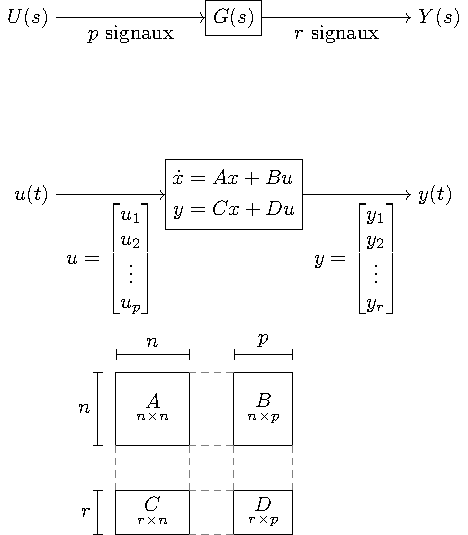
\includegraphics[scale=1,page=1]{drwg_0.pdf}
\end{figure}
\subsection{$A,B,C,D \longrightarrow G$}
$$G(s)=C(sI-A)^{-1}B+D$$
$$G(z)=C_n(zI-A_n)^{-1}B_n+D_n$$
\subsubsection{Gain haute fréquence}
$$\lim_{s\to\infty}G(s)=D$$
\subsubsection{Gain basse fréquence}
$$G(0)=-CA^{-1}B+D$$

\subsection{$G(s)\longrightarrow A,B,C,D$}
\subsection{$G(z)\longrightarrow A,B,C,D$}

\subsection{Mise en cascade}
\begin{figure}[H]
\centering
\includegraphics[scale=1,page=2]{drwg_0.pdf}
\end{figure}
$$S_{tot}=S_2(s)\cdot S_1(s)\qquad\text{ordre important}$$
$$A_{tot}=\begin{bmatrix}
A_1 & 0\\
B_2C_1 & A_2
\end{bmatrix}\qquad B_{tot}=\begin{bmatrix}
B_1\\B_2D_1
\end{bmatrix}$$
$$C_{tot}=\begin{bmatrix}
D_2C_1 & C_2
\end{bmatrix}\qquad D_{tot}=D_2D_1$$
\subsection{Mise en parallèle}
\begin{figure}[H]
\centering
\includegraphics[scale=1,page=3]{drwg_0.pdf}
\end{figure}
$$S_{tot}(s)=S_1(s)+S_2(s)$$
$$A_{tot}=\begin{bmatrix}
A_1 & 0\\0 & A_2
\end{bmatrix}\qquad B_{tot}=\begin{bmatrix}
B_1\\B_2
\end{bmatrix}$$
$$C_{tot}=\begin{bmatrix}
C_1 & C_2
\end{bmatrix}\qquad D_{tot}=D_1+D_2$$
\subsubsection{Mise en contre-réaction 1}
\begin{figure}[H]
\centering
\includegraphics[scale=1,page=4]{drwg_0.pdf}
\end{figure}
$$A_{tot}=\begin{bmatrix} A_1 - B_1D_2(I-D_1D_2)^{-1}C_1 & -B_1(C_2-D_2D_1C_2)\\B_2(I-D_1D_2)^{-1}C_1 & A_2-B_2(I-D_1D_2)^{-1}D_1C_2\end{bmatrix}\qquad B_{tot}=\begin{bmatrix}B_1-B_1D_2ND_1\\B_2ND_1\end{bmatrix}$$

$$C_{tot}=\begin{bmatrix}(I-D_1D_2)^{-1}C_1 & -(I-D_1D_2)^{-1}D_1C_2\end{bmatrix}\qquad D_{tot}=(I-D_1D_2)^{-1}D_1$$ 

\subsubsection{Mise en contre-réaction 2}
\begin{figure}[H]
\centering
\includegraphics[scale=1,page=5]{drwg_0.pdf}
\end{figure}
$$S_{tot}(s)=\left(I+S_1(s)S_2(s)\right)^{-1}S_1(s)$$
$$A_{tot}=\begin{bmatrix}A_1 & 0\\B_2C_1 & A_2\end{bmatrix}\qquad B_{tot}=\begin{bmatrix}B_1\\B_2D_1\end{bmatrix}$$
$$C_{tot}=\begin{bmatrix}
D_2 C_1 & C_2
\end{bmatrix}\qquad D_{tot}=D_1D_2$$
\end{document}